\documentclass[dvipdfmx]{jsarticle}
\usepackage[dvipdfmx]{graphicx}
\usepackage{amsmath, amssymb}
\usepackage{mathtools}
\usepackage{here}

\begin{document}
\title{}
\author{権藤陸}
\maketitle

\section*{ノイズについて}

以下にウェーブレット再構成前後におけるWelch法で得た周波数特性(0-3.0Hz)を示します.
次の式で定義するウェーブレット再構成前と後の平均パワー比を求めると,
\begin{equation}\label{}
平均パワー比 = \frac{0-0.6 \mathrm{Hz}の平均パワー}{0.6-2 \mathrm{Hz}の平均パワー}
\end{equation}

心拍に起因する周波数0.6-2 Hz以外の周波数帯の信号をノイズと仮定します.
ウェーブレット再構成前は平均パワー比が980.6, ウェーブレット再構成後は平均パワー比が5.2で,再構成後の方がパワー比が約1/189になり,0.6Hz未満のノイズがウェーブレット再構成によって抑えられたため,モデルの学習が安定し,良い精度が出たのではないかと考えられます.

\begin{figure}[htbp]
    \begin{minipage}[c]{0.5\hsize}
      \centering
      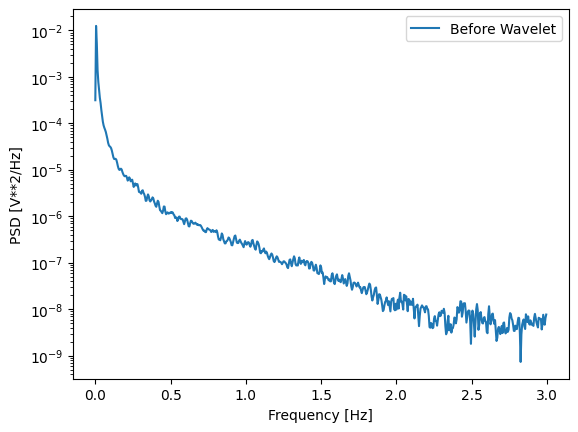
\includegraphics[width=\linewidth]{./img/before_wavelet_freq.png}
      \caption{ウェーブレット再構成前の周波数特性(Welch法)}
    %   \label{fig:statue}
    \end{minipage}
    \begin{minipage}[c]{0.5\hsize}
      \centering
      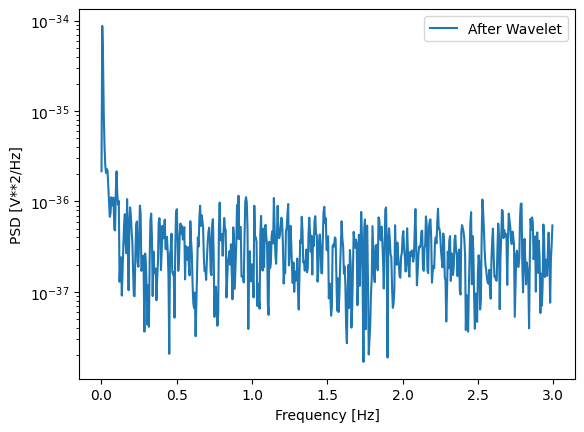
\includegraphics[width=\linewidth]{./img/after_wavelet_freq.png}
      \caption{ウェーブレット再構成後の周波数特性(Welch法)}
    %   \label{fig:spaceship}
    \end{minipage}
\end{figure}

\begin{table}[H]
\caption{Welch法のパラメータ}
\centering
\begin{tabular}{cc}
\hline
全体のウィンドウサイズ & 200000 \\
セグメントあたりのポイント数 & 50000 \\
オーバーラップ & 25000 \\
周波数分解能(Hz) & 0.005 \\
サンプリングレート(s) & 250 \\
\hline
\end{tabular}
\end{table}

\newpage

以下にウェーブレット再構成前後の,ある5秒セグメントのSTFTの結果を示します.
左はウェーブレット再構成前,右はウェーブレット再構成後です.
STFTの結果からは,ウェーブレット再構成後の方が,2Hz以上の信号のパワーが比率的に高い程度しか得られる情報はありませんでした.

\begin{figure}[htbp]
    \begin{minipage}[c]{0.5\hsize}
      \centering
      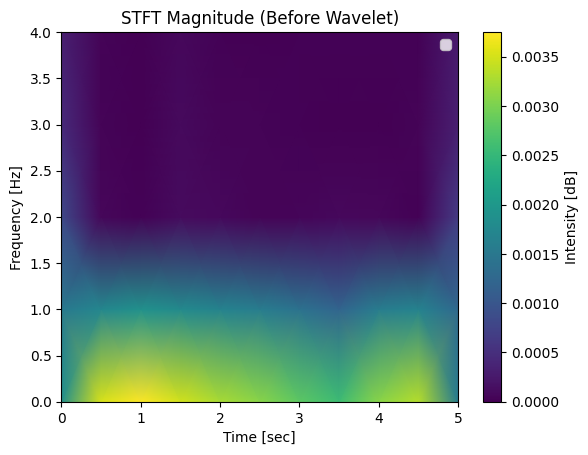
\includegraphics[width=\linewidth]{./img/stft_before.png}
      \caption{ウェーブレット再構成前のスペクトログラム}
    %   \label{fig:statue}
    \end{minipage}
    \begin{minipage}[c]{0.5\hsize}
      \centering
      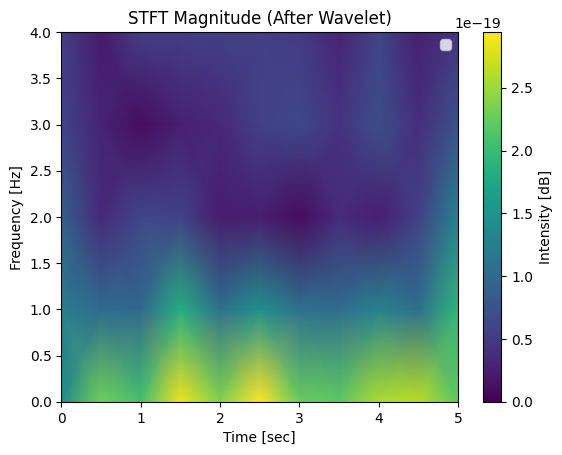
\includegraphics[width=\linewidth]{./img/stft_after.png}
      \caption{ウェーブレット再構成後のスペクトログラム}
    %   \label{fig:spaceship}
    \end{minipage}
\end{figure}

\begin{table}[H]
    \caption{STFTのパラメータ}
    \centering
    \begin{tabular}{cc}
    \hline
    全体のウィンドウサイズ & 1250 \\
    セグメントあたりのポイント数 & 250 \\
    オーバーラップ & 125 \\
    サンプリングレート(s) & 250 \\
    \hline
    \end{tabular}
\end{table}


\end{document}